\section*{Fields of Order \(p^n\) : \(\GF(p^n)\)}

We saw that if a finite field of order \(p^n\) is given, it is isomorphic to the zeros of \(x^{p^n} - x \in \Z_p[x]\). Now we want to see if a field of order \(p^n\) exists for any given \(p\) and \(n\).

We have two candidates. If there exists an irreducible polynomial \(f(x)\) of degree \(n\) over \(\Z_p\), we know that \(\Z_p[x] \quotient \span{f(x)}\) is a finite field of order \(p^n\). Or we can try to show that the zeros of \(x^{p^n} - x\) form a field.

\lemma{1} \(x^{p^n} -x \in \Z_p[x]\) has \(p^n\) distinct zeros in \(\bar{\Z_p}\).

\pf Since the polynomial has degree \(p^n\) and \(0\) is a zero, we show that \(x^{p^n - 1} - 1\) has \(p^n - 1\) distinct zeros. Suppose that \(\alpha \in \bar{\Z_p}\) is a zero of \(x^{p^n - 1} - 1\). Then
\[\tag{\mast}
    \frac{x^{p^n - 1} - 1}{x - \alpha} = x^{p^n - 2} + \alpha x^{p^n-3} + \cdots + \alpha^{p^n - 2}.
\]
Set \(x = \alpha\), then (\mast) is equal to \((p^n - 1)\alpha^{p^n - 2} = -\alpha\inv \neq 0\), thus \(\alpha\) cannot be a multiple root. \qed

\lemma{2} If \(\alpha, \beta\) are zeros of \(x^{p^n} - x\), then \(\alpha \pm \beta\), \(\alpha\beta\), \(\alpha/\beta\) are also zeros of \(x^{p^n} - x\).

\pf Trivial. \qed

\thm. Let \(p\) be prime, and \(n \in \N\). Then there exists a field of order \(p^n\).

Thus, given a finite field \(F\), we can extend \(F\) with given dimension. Then the extension field \(E\) is a finite extension, thus \(E\) is a simple extension.

\cor. Let \(F\) be a finite field. For \(n \in \N\), there exists a irreducible polynomial \(p(x) \in F[x]\) of degree \(n\).

\pf Let \(\ch F = p\), then \(\abs{F} = p^r\) for some \(r \in \N\). Since elements of \(F\) are zeros of \(x^{p^r} - x\), we have \(\alpha^{p^{rn}} = \alpha\) for \(\alpha \in F\). Consider a finite field \(K\) of order \(p^{rn}\). Then \(\alpha \in K\), so \(F \leq K\). \(K\) is a finite extension of \(F\), so \(K\) must be a simple extension of degree \(n\). There is an element \(\beta \in K\) such that \(K = F(\beta)\), so \(\irr(\beta, F)\) is the polynomial we're looking for. \qed

Our next question is the uniqueness!

\thm. Let \(E, E'\) be fields of order \(p^n\). Then \(E \simeq E'\).

\pf \(E \simeq \Z_p[x] \quotient \span{p(x)}\) where \(p(x) \in \Z_p[x]\) is irreducible with degree \(n\). For any \(\alpha \in E\), \(\alpha^{p^n} - \alpha = 0\), so \(p(x) \mid (x^{p^n} - x)\). In addition, \(E'\) also consists of zeros of \(x^{p^n} - x\), so \(E'\) has zeros of \(p(x)\). Since \(E'\) has order \(p^n\), then we have \(E' \simeq \Z_p[x] \quotient \span{p(x)} \simeq E\). \qed

Conclusion. For a prime \(p\) and \(n \in \N\), there exists a unique field of order \(p^n\), up to isomorphism. Furthermore, this field is a simple extension field of order \(p^m\) (\(m < n\)), and contains zeros of \(x^{p^n} - x \in \Z_p[x]\).

\pagebreak

\setcounter{chapter}{6}

\chapter{Advanced Group Theory}

We briefly review advanced group theory from last semester.

\setcounter{topic}{33}
\topic{Isomorphism Theorems}

\thm. \note{First Isomorphism Theorem} Let \(\varphi : G \ra G'\) be a group homomorphism. Then \(\bar{\varphi} : G \quotient \ker \varphi \ra \im \varphi\) defined as
\[
    \bar{\varphi}(\bar{x}) = \varphi(x), \quad (x \in G)
\]
is an isomorphism, and \(G \quotient \ker \varphi \simeq \im \varphi\).
\[
    \begin{tikzcd}
        G \arrow{rr}{\varphi} \arrow[swap]{dr}{\pi} & \arrow[d, phantom, "\circlearrowright"]& \im \varphi \\
        & G \quotient \ker\varphi \arrow[dashed,swap]{ur}{\bar{\varphi}} &
    \end{tikzcd}
\]

\thm. \note{Second Isomorphism Theorem} If \(H \leq G\) and \(N \nsub G\),
\[
    \frac{HN}{N} \simeq \frac{H}{H\cap N}.
\]
\begin{center}
    \begin{tikzpicture}
        \node (H) at (0, 0) {\(H\)};
        \node (HN) at (3, 0) {\(HN\)};
        \node (HoverHcapN) at (0, -2.5) {\(\dfrac{H}{H \cap N}\)};
        \node (HNoverN) at (3, -2.5) {\(\dfrac{HN}{N}\)};

        \draw[->] (H) -- (HN) node[midway,above,scale=0.7] {\(\imath\)};
        \draw[->] (HN) -- (HNoverN) node[midway,right,scale=0.7] {\(\pi'\)};
        \draw[->] (H) -- (HoverHcapN) node[midway,left,scale=0.7] {\(\pi\)};
        \draw[->] (HoverHcapN) -- (HNoverN) node[midway,below,scale=0.7] {\(\bar{\jmath}\)} node[midway,above,scale=0.7] {\(\simeq\)};
        \draw[->] (H) -- (HNoverN) node[midway,above right,scale=0.7] {\(\jmath\)};

        \node[scale=0.6] at (0.7, -1.6) {\(\circlearrowright\)};
        \node[scale=0.6] at (2.3, -0.6) {\(\circlearrowright\)};
    \end{tikzpicture}
\end{center}

\thm. \note{Third Isomorphism Theorem} If \(H, K \nsub G\) and \(K \leq H\),\footnote{This implies that \(K \nsub H\).} then
\[
    G \quotient H \simeq \frac{G \quotient K}{H \quotient K}.
\]

\topic{Series of Groups}

\defn. Given a \textit{finite} sequence of subgroups
\[
    \{e\} = H_0 < H_1 < \cdots < H_k = G,
\]
\begin{enumerate}
    \item \note{Subnormal Series} If \(H_i \pnsub H_{i+1}\) for \(i = 0, \dots, k - 1\), it is called a \textbf{subnormal series}.
    \item \note{Normal Series} If \(H_i \pnsub G\) for \(i = 0, \dots, k - 1\), it is called a \textbf{normal series}.
\end{enumerate}

\rmk Since \(H_i \pnsub G \implies H_i \pnsub H_{i+1}\), a normal series is a subnormal series.

We want to decompose a group \(G\) into normal subgroups. We focus on the quotient groups that appear in the series.

\defn. \note{Refinement} For two subnormal (normal) series \(\seq{H_i}\) and \(\seq{K_j}\) of \(G\), \(\seq{K_j}\) is a \textbf{refinement} of \(\seq{H_i}\) if \(\seq{H_i} \subset \seq{K_j}\).

\defn. Subnormal (normal) series \(\seq{H_i}_{i \in I}\), \(\seq{K_j}_{j \in J}\) of \(G\) are \textbf{isomorphic} if there exists a bijection between
\[
    \{H_{i+1} / H_i\} \longleftrightarrow \{K_{j+1} / K_j\}
\]
such that the corresponding quotient groups are isomorphic.

\thm. \note{Schrier} Any two subnormal (normal) series of \(G\) have isomorphic refinements.

\defn. Let \(\seq{H_i}\) be a subnormal (normal) series of \(G\). If \(H_{i+1} \quotient H_i\) is simple for any \(i\), \(\seq{H_i}\) is called a \textbf{composition (principal) series}.

\thm. \note{Jordan-Hölder} Any two composition series of a group \(G\) are isomorphic.

\defn. \note{Solvable Group} A group \(G\) is \textbf{solvable} if there exists a composition series \(\seq{H_i}\) such that all quotient groups are abelian.

\pagebreak
